\newpage
\section{Natalia Kwiecień}

Math expression:

\[sin(2\alpha) = 2sin(\alpha)cos(alpha) \]

Table~\ref{tab:sheep per capita} represents number of sheep per capita in countries with more sheep than people

\vspace{0.1cm}

\begin{table}[htbp]
\begin{tabular}{llll}
Country          & Population & Number of sheep & Number of sheep per capita \\
Iceland          & 360k       & 454k            & 1.2                        \\
Ireland          & 5M         & 5.5M            & 1.1                        \\
Wales            & 3.1M       & 9.5M            & 3                          \\
Mongolia         & 3.3M       & 14.8M           & 4.5                        \\
New Zealand      & 5M         & 38.4M           & 7.7                        \\
Falkland Islands & 3.5k       & 700k            & 200                       
\end{tabular}
\label{tab:sheep per capita}
\end{table}

Captured by NASA’s James Webb Space Telescope, this image reveals previously obscured areas of star birth. (see Figure~\ref{fig:Cosmic cliffs}).

\vspace{0.1cm}

\begin{figure}[htbp]
    \centering
    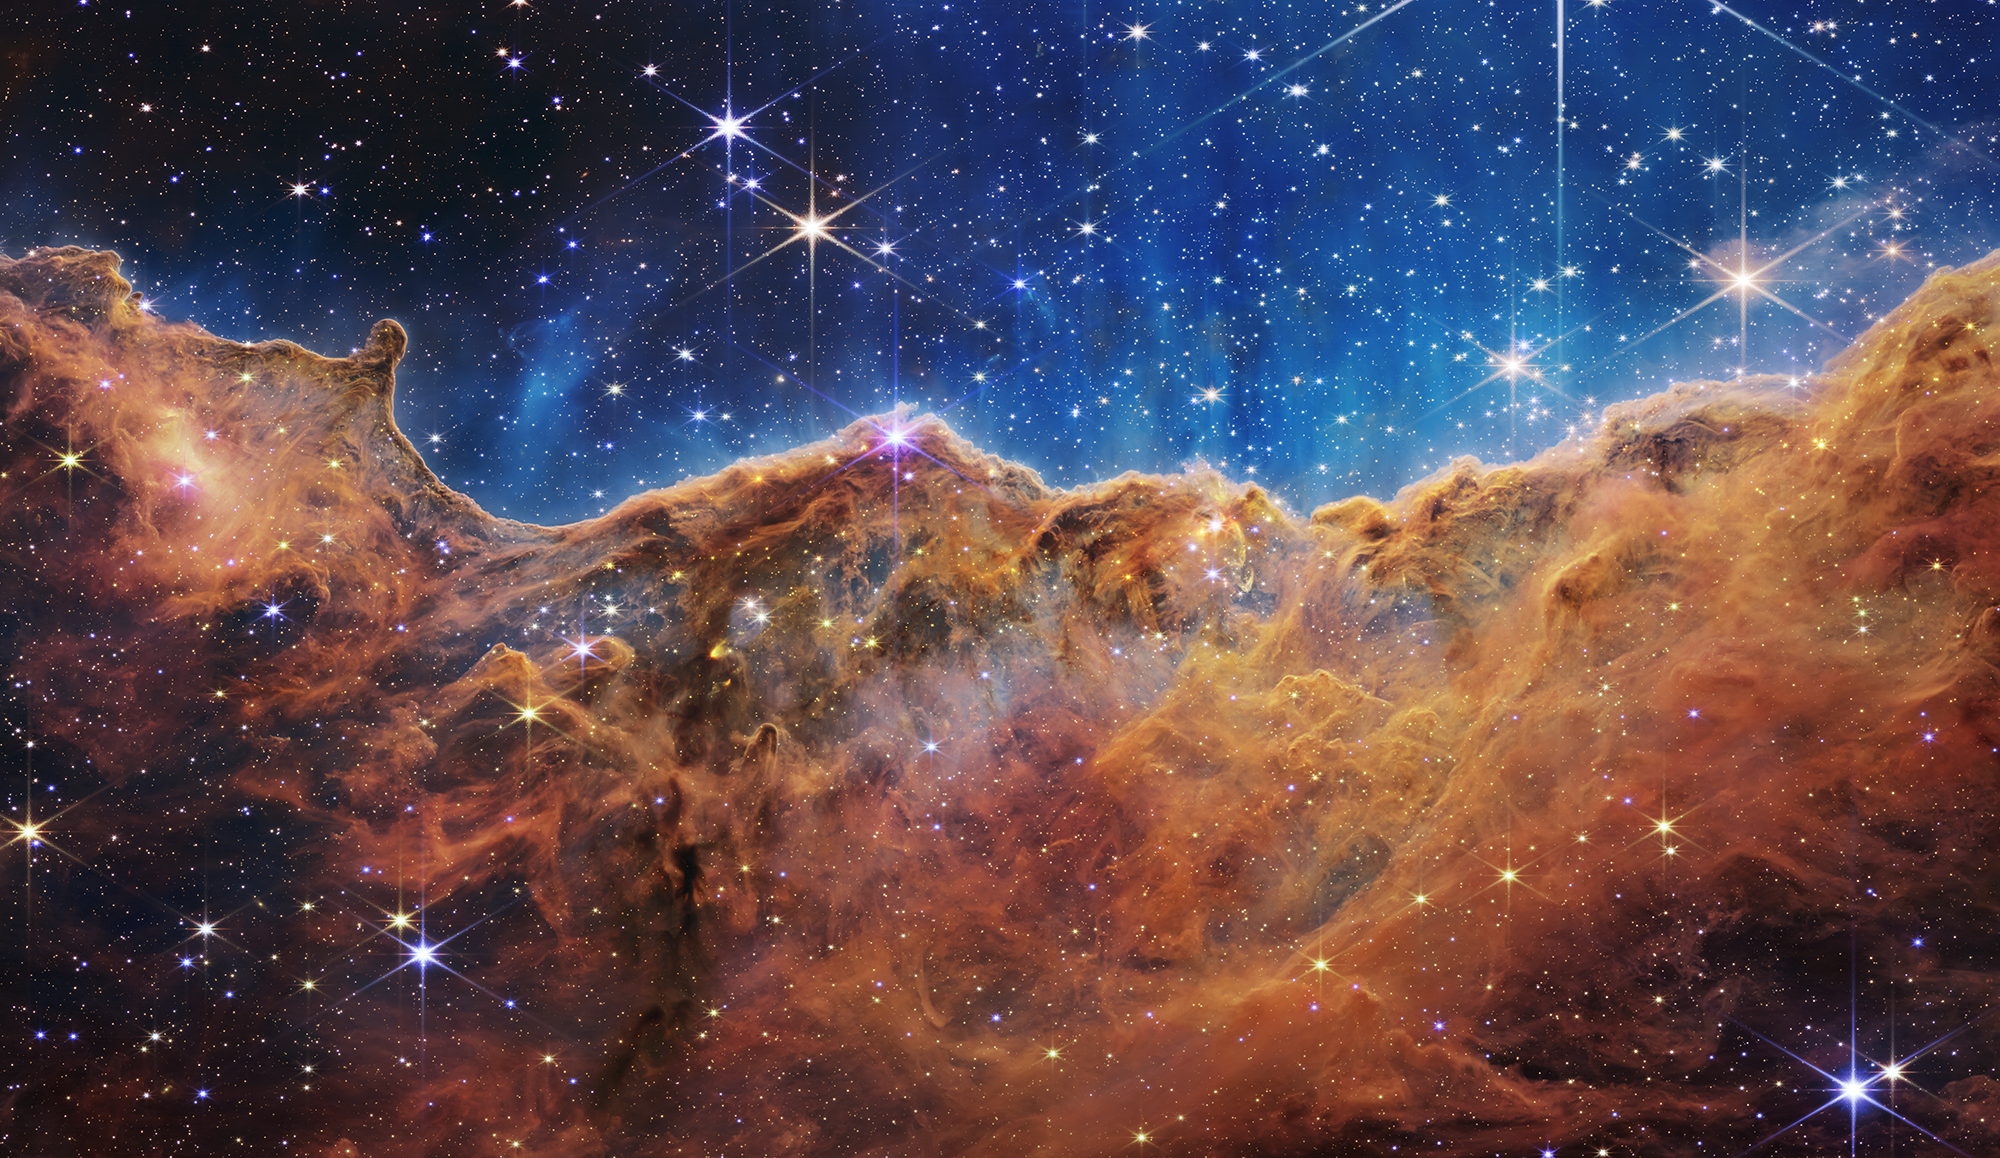
\includegraphics[width=0.8\textwidth]{Pictures/Cosmic cliffs.png} 
    \caption{A star was born}
    \label{fig:Cosmic cliffs}
\end{figure}

\begin{align} 
\textbf{Pierwszy utwór najlepszego albumu wszechczasów Tranquility Base Hotel and Cassino autorstwa Arctic Monkeys}

\vspace{0.1cm}

Star Treatment to wprowadzenie do albumu; Alex zaczyna
przedstawienie siebie i tego, co sprowadziło go to hotelu. Jest artystą z lat 70, który 
{nie może już odnaleźć się na Ziemi i postanawia obserwować ją z księżyca.} Jest to los, który spotyka wielu celebrytów. Już tytuł wskazuje, że hotel jest miejscem, które ma pomóc uciec od świata i się „wyleczyć” (raczej nieskutecznie). Tak naprawdę dopiero w kolejnych piosenkach zgłębia kierunek, do którego dąży nasz świat; tutaj raczej subtelnie o tym wspomina, zwłaszcza nawiązując do \emph{Blade Runnera} czy \emph{Orwella 1984}.

\end{align}
\vspace{0.1cm}

\begin{align} 

\underline{I just wanted to be one of The Strokes} \\
\underline{Now look at the mess you made me make} \\

Alex wspomina początki swojej kariery i jak sam powiedział \empth{pierwszy wers miał być czymś, co mógłby napisać w pierwszym albumie Arctic Monkeys}. Początkowo pierwsze wersy nie miały nawet trafić do albumu, jednak mając w głowie koncept powrotu do przeszłości, postanowił go zostawić. Pokazuje, co ostatecznie sprowadziło go daleko od Ziemi.

\end{align}
\vspace{0.1cm}

\begin{align}

\underline{Love came in a bottle with a twist-off cap} \\
\underline{Let's all have a swig and do a hot lap} \\

TBH&C ma służyć przyjemności jednak nic nie jest tam „autentyczne” ​
i \emph{nawet miłość może być przepisana w formie tabletek}. „Hot lap” jest bardzo sprytnym sformułowaniem, bo poza oczywistym znaczeniem, a tego co zrozumiałam oznacza szybki „wyścig” samochodów, który nie ma wielkiego znaczenia, ponieważ nikt go nie wygrywa. Tak jak uczucia nie mają tam już znaczenia.

\end{align}
\vspace{0.1cm}

List of coutries with more cattle than people:
\begin{enumerate}
    \item Uruguay	
    \item New Zealand	
    \item Argentina     
    \item Australia	
    \item Brazil	
    \item Colombia
    \item Belarus
    \item Venezuela
    \item Canada
    \item United States
    \item India
    \item EU
    \item Mexico
    \item Russia
    \item Ukraine
    \item China
    \item Egypt
    \item South Korea
    \item Japan
\end{enumerate}

Best artists according to me:
\begin{itemize}
  \item Arctic Monkeys
  \item Lana del Rey
  \item David Bowie
  \item Mitski
\end{itemize}
